\documentclass[12pt]{article}
\usepackage{amsmath} % flere matematikkommandoer
\usepackage[utf8]{inputenc} % æøå
\usepackage[T1]{fontenc} % mere æøå
\usepackage[danish]{babel} % orddeling
\usepackage{verbatim} % så man kan skrive ren tekst
\usepackage[all]{xy} % den sidste (avancerede) formel i dokumentet
\usepackage{amsmath}
\usepackage{amsfonts}
\usepackage{amssymb}
\usepackage{graphicx}
\usepackage{fancyhdr}
\usepackage{moreverb}


\title{Algorithms and Datastructures assignment 1}
\author{Thomas Broby Nielsen}

\begin{document}
\maketitle

\tableofcontents

\pagebreak
\section{Task 1}
1)
\\
$
p(n)=8p(n/2)+n^{2}
$\\
$a=8$ $b=2$ $f(n)=n^{2}$ $n^{log_{b}a}=n^{log_{2}8}=n^3$\\
since $n^{log_28}=n^3$ some constant $\epsilon > 0 $ exists so $n^2=O(n^{log_2(8-\epsilon)})$ is true. We use case 1 of the master theorem\\
Thus $p(n)=\Theta (n^3)$\\
\\
2)
\\
$p(n)=8p(n/4)+n^{3}\\$
$a=8$ $b=4$ $f(n)=n^{3}$ $n^{log_{b}a}=n^{log_{4}8}=n^{3/2}$\\
since $n^{log_48}=n^3$ some constant $\epsilon > 0$ exists so $n^3=\Omega(n^{log_4(8+\epsilon)})$  is true. We use case 3 of the master theorem\\
And $8 \frac {n^3}{4^3} \leq cn^3$ and c < 1 =\\
 $8 \frac {n^3}{64} \leq cn^3$ and c < 1 =\\
 $ \frac {n^3}{8} \leq cn^3$ and c < 1 =\\
 $ \frac {1}{4}n \leq cn^3$ and c < 1 =\\
 $  \frac {1}{4} \leq c$=\\
Thus $p(n)=\Theta(n^3)$\\
\\
3)
\\
$p(n)10p(n/9)+nlog_2n$
\\
$a=10$, $b=9$ $\rightarrow$ $f(n)=nlog_2n$ $n^{log_{b}a}=n^{log_910}=n^{1.04795}$
\\
Since $n^{log_910}$ is an exponential expression with a power > 1, and $n log_2 n$ is a logarithmic expression, $n^{log_910}$ will eventually be larger than $n log_2 n$ for a big enough n
\\
Thus $n log_2 n = O(n^{log_910-\epsilon})$ is true for a small enough $\epsilon$ and a big enough n.
$p(n)=\Theta (n^{log_910}).$
\newpage
\section{task 2}
From the function given to us in this task ($p(n) = p(\frac{n}{2}) p(\frac{n}{3}) + n$), we have constructed the following tree to show the growth of the function.
\begin{figure}[!h]
 	\begin{center}
	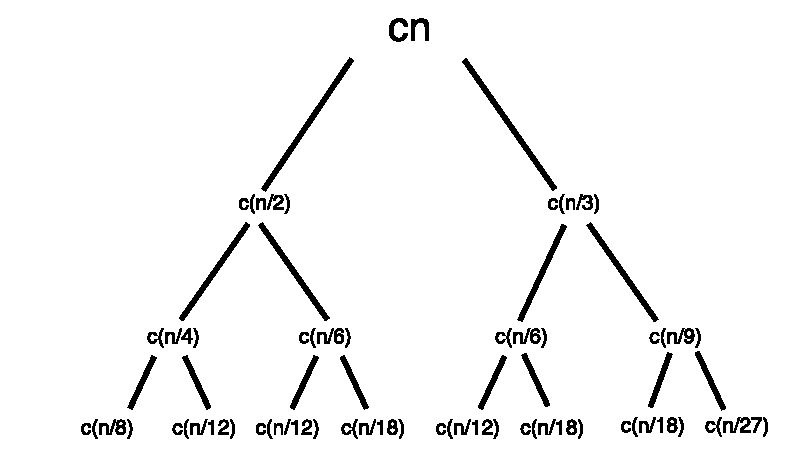
\includegraphics[scale=1]{include/Tree_diagram}
	\end{center}
	\caption{Diagram over the tree structur of the $p(n) = p(\frac{n}{2}) + p(\frac{n}{3}) + n)$ function.}
	\label{Sekvens-user}
\end{figure}
From this we have made the edjucated guess that our recursive function $p(n) = p(\frac{n}{2}) p(\frac{n}{3}) + n $ has the running time of $O(n \cdot lgn)$.


\section{Task 3}
Bellow we have written the pseudo-code for Introsort. The functions Heapsort, Insertionsort, and Randomized-partition is from CLRS\\

\begin{verbatim}
1 int RecursionDepth = 0
2 int c = 16 or 32
3	
4 IntroSort (A, i, j,)
5    if j - i > c 
6       if recursionDepth > 2log(j-i)
7         HeapSort(A[i,j])
8       else 
9            RecursionDepth++
10           q = RandomizedPartition (A, i, j)
11           IntroSort(A, i, q-1)
12           IntroSort(A, q+1, j)
13   else 
14        Insertion
Sort(A[i,j])
\end{verbatim}
\section{Task 4}
Introsort has a worst case runtime of O(n log n) because Quicksort\cite{introduction-algorithms} (which has a worst case runtime of O(n2)) is replaced with Heapsort\cite{introduction-algorithms} (which has a worst runtime of O(n log n) if it's recursiondepth becomes too big. thus the worst case will never happen. 
InsertionSort\cite{introduction-algorithms} also has a worst case runtime of O(n2), but it is used on an almost already sorted array which it is very efficient at.

\section{Task 5}
unlike merge sort, heapsort sorts in place: only a constant number of array elements are stored outside the input array at any time. This makes it more memory efficient. 

\section{Task 6}
Insertion sort has a best case runtime of O(n) making it potentially much faster than the other sorting algorithms. the best case for Insertion sort is when the array is already sorted, so letting it sort an already almost sorted array will give a runtime close to its best case.

\bibliographystyle{plain}
\bibliography{references}
\end{document}